\section{Transformer GAN}

Even though with our last model we could be able to achieve good results in terms of metric scores, we wanted to develop at least one adversarial model \cite{goodfellow2014generative} in order to try getting rid of the \texttt{categorical crossentropy} loss function, which could not always be a good choice for the particular task we were intended to solve.

\begin{figure}[!htb]
    \centering
    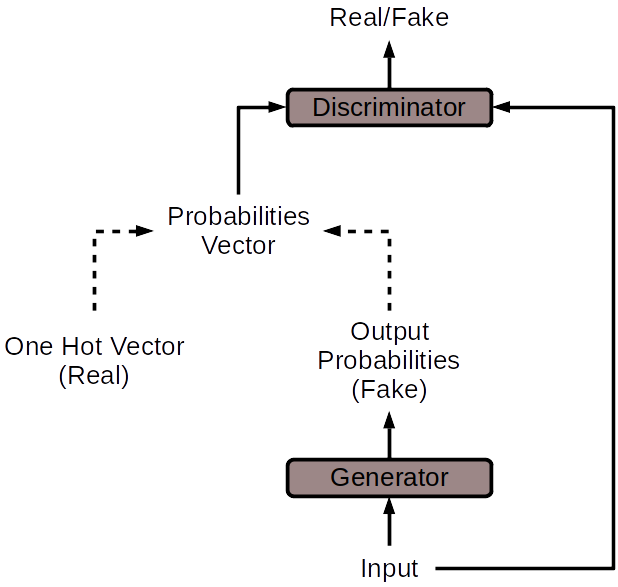
\includegraphics[scale=0.65]{images/model-6-general.png}%
    \caption{Overall GAN Architecture}%
    \label{gan-general}
\end{figure}

Overall, our architecture, as depicted in figure \ref{gan-general}, is composed of a \texttt{\textsc{Generator}} and a \texttt{\textsc{Discriminator}}.
The former takes as input a fixed-length sample of the \textit{Divine Comedy}, as well as the standard \textit{RNN} models and the first version of the \textit{Transformer}, while returning as output a vector of probabilities for the next sample.
Instead, the latter is a \textit{Siamese Network} taking as input both that sample and either the output probabilities vector of the \texttt{\textsc{Generator}} or the one-hot encoded vector representing the actual token.
A closer look of the two modules is presented in the figure \ref{gan-specific}.

\begin{figure}[!htb]
    \centering
    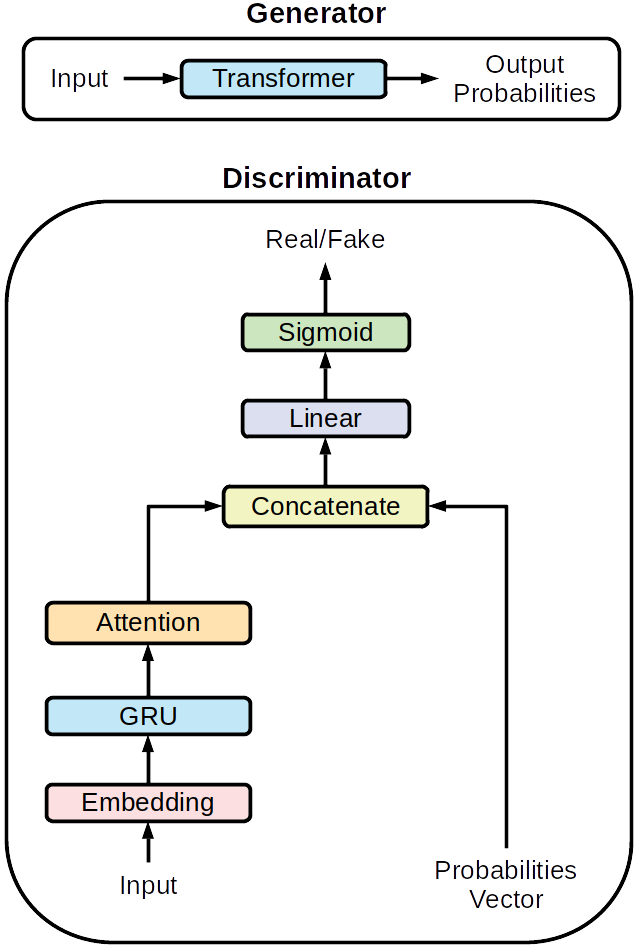
\includegraphics[scale=0.6]{images/model-6-specific.png}%
    \caption{Generator \& Discriminator of the GAN Architecture}%
    \label{gan-specific}
\end{figure}

The reason why we had to switch back to the previous way of splitting the text instead of going on with the verse-level division is that, during the training, it was not possible to generate an entire verse (made up of multiple tokens) at once without having to apply an \textit{hardmax} activation to the generated vectors.
Thus, being the \textit{hardmax} activation non-linear, this would have made impossible to get the gradients related to the weights of the net and, subsequently, to correctly perform the backpropagation step.

\subsubsection{\textsc{Hyperparameters and Results}}

Both the \texttt{\textsc{Generator}} and the \texttt{\textsc{Siamese Discriminator}} had their own hyperparameters to be set.
In particular, those of the \texttt{\textsc{Generator}} are:
\begin{itemize}
    \item the number of layers of the \textit{Transformer}
    \item the number of heads  of the \textit{Transformer}
    \item the dimensions of the latent spaces (\texttt{d\_model} and \texttt{dff})
    \item the dropout
\end{itemize}
while, those of the \texttt{\textsc{Discriminator}} are:
\begin{itemize}
    \item the \textsc{Embedding} dimension
    \item the number of \textsc{GRU} units
    \item the \textsc{Attention} kind
    \item the \textsc{GRU} dropout
\end{itemize}

Even though we tried some different kind of settings, we could never reach the \textit{Nash Equilibrium} between the two modules of the \textit{GAN}\footnote{
    Generally, the \texttt{\textsc{Generator}} seemed to be more powerful than the \texttt{\textsc{Discriminator}}, even for those cases in which we largely reduced its size.
}, which prevented us from having any fit sample at all.

Given that finding an equilibrium during an adversarial train is a well-known complex problem in the field of \textit{Deep Learning}, and that the methods to overcome it require a deep knowledge of many \textit{state-of-the-art} techniques, we decided to stop our investigations here, also given that the results of our previous model were good enough in our opinion.
Anyhow, we shall at least briefly present some of these techniques in the next chapter.